% begin module inverse-function-ex5
\begin{frame}
\begin{example}%[Example 5, p. 388]
\begin{columns}[c]
\column{.5\textwidth}
\ \only<handout:0| -1>{%
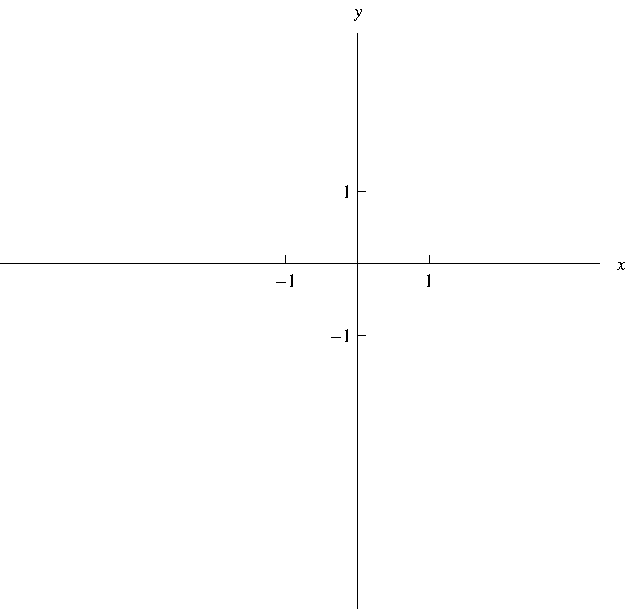
\includegraphics[height=4.5cm]{inverse-functions/pictures/07-01-ex5a.pdf}%
}%
\only<handout:0| 2>{%
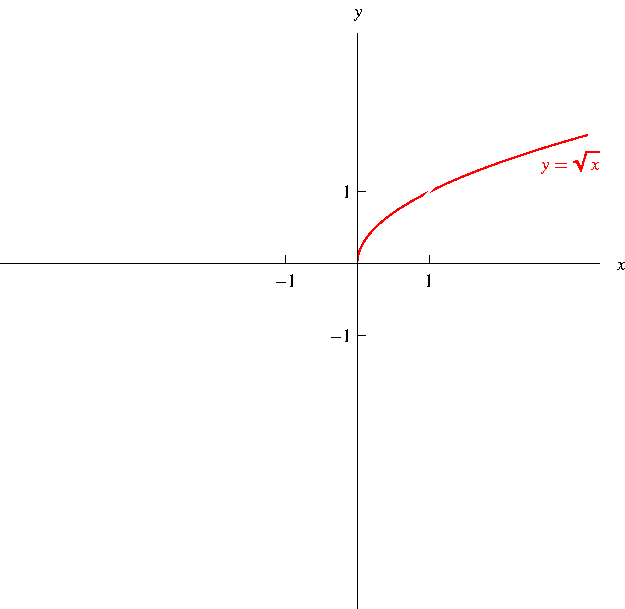
\includegraphics[height=4.5cm]{inverse-functions/pictures/07-01-ex5b.pdf}%
}%
\only<handout:0| 3>{%
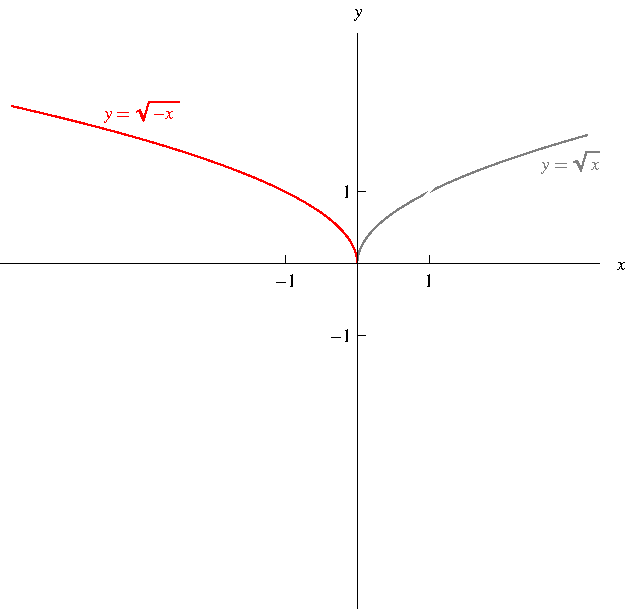
\includegraphics[height=4.5cm]{inverse-functions/pictures/07-01-ex5c.pdf}%
}%
\only<handout:0| 4>{%
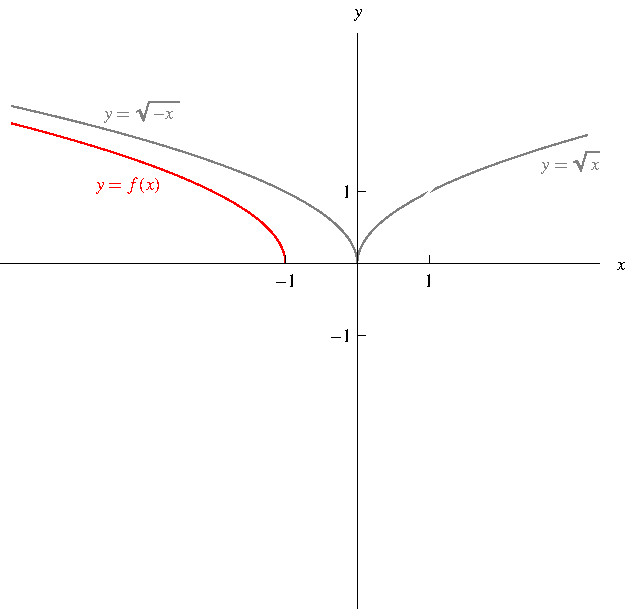
\includegraphics[height=4.5cm]{inverse-functions/pictures/07-01-ex5d.pdf}%
}%
\only<handout:1| 5->{%
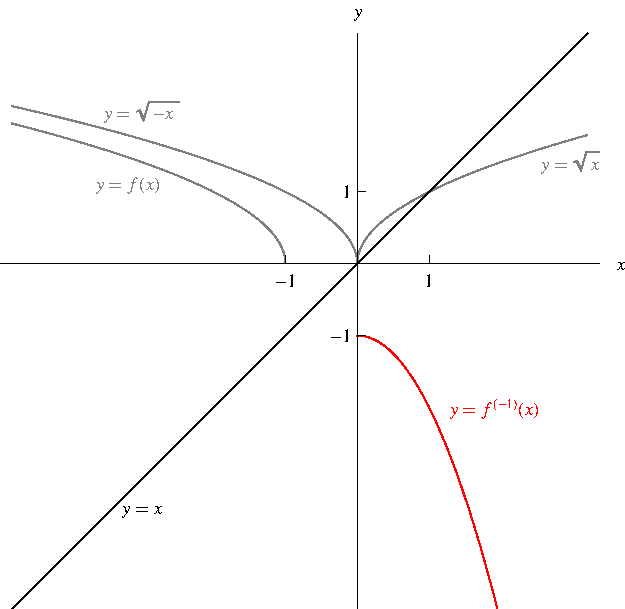
\includegraphics[height=4.5cm]{inverse-functions/pictures/07-01-ex5e.pdf}%
}%
\column{.5\textwidth}
Sketch the graph of $f(x) = \sqrt{-x - 1}$ and its inverse function.
\end{columns}
\begin{itemize}
\item<2->  First draw the graph of $y = \sqrt{x}$.
\item<3->  $y = \sqrt{-x}$ is the reflection of $y = \sqrt{x}$ in the $y$-axis.
\item<4->  $y = f(x) = \sqrt{-x - 1}$ is the shift of $y = \sqrt{-x}$ one unit to the left.
\item<5->  $y = f^{-1}(x)$ is the reflection of $y = f(x)$ in the line $y = x$.
\end{itemize}
\end{example}
\end{frame}
% end module inverse-function-ex5
